\section{Stabilizer}
Previously it was shown that the dynamics of a humanoid robot can be a single inverted pendulum and how the pendulum maintains a desired position thanks to the controller designed. Now, let us introduce the detailed stabilizer structure (Figure \ref{fig:stabilizer}).

\begin{figure}[!h]
\centering
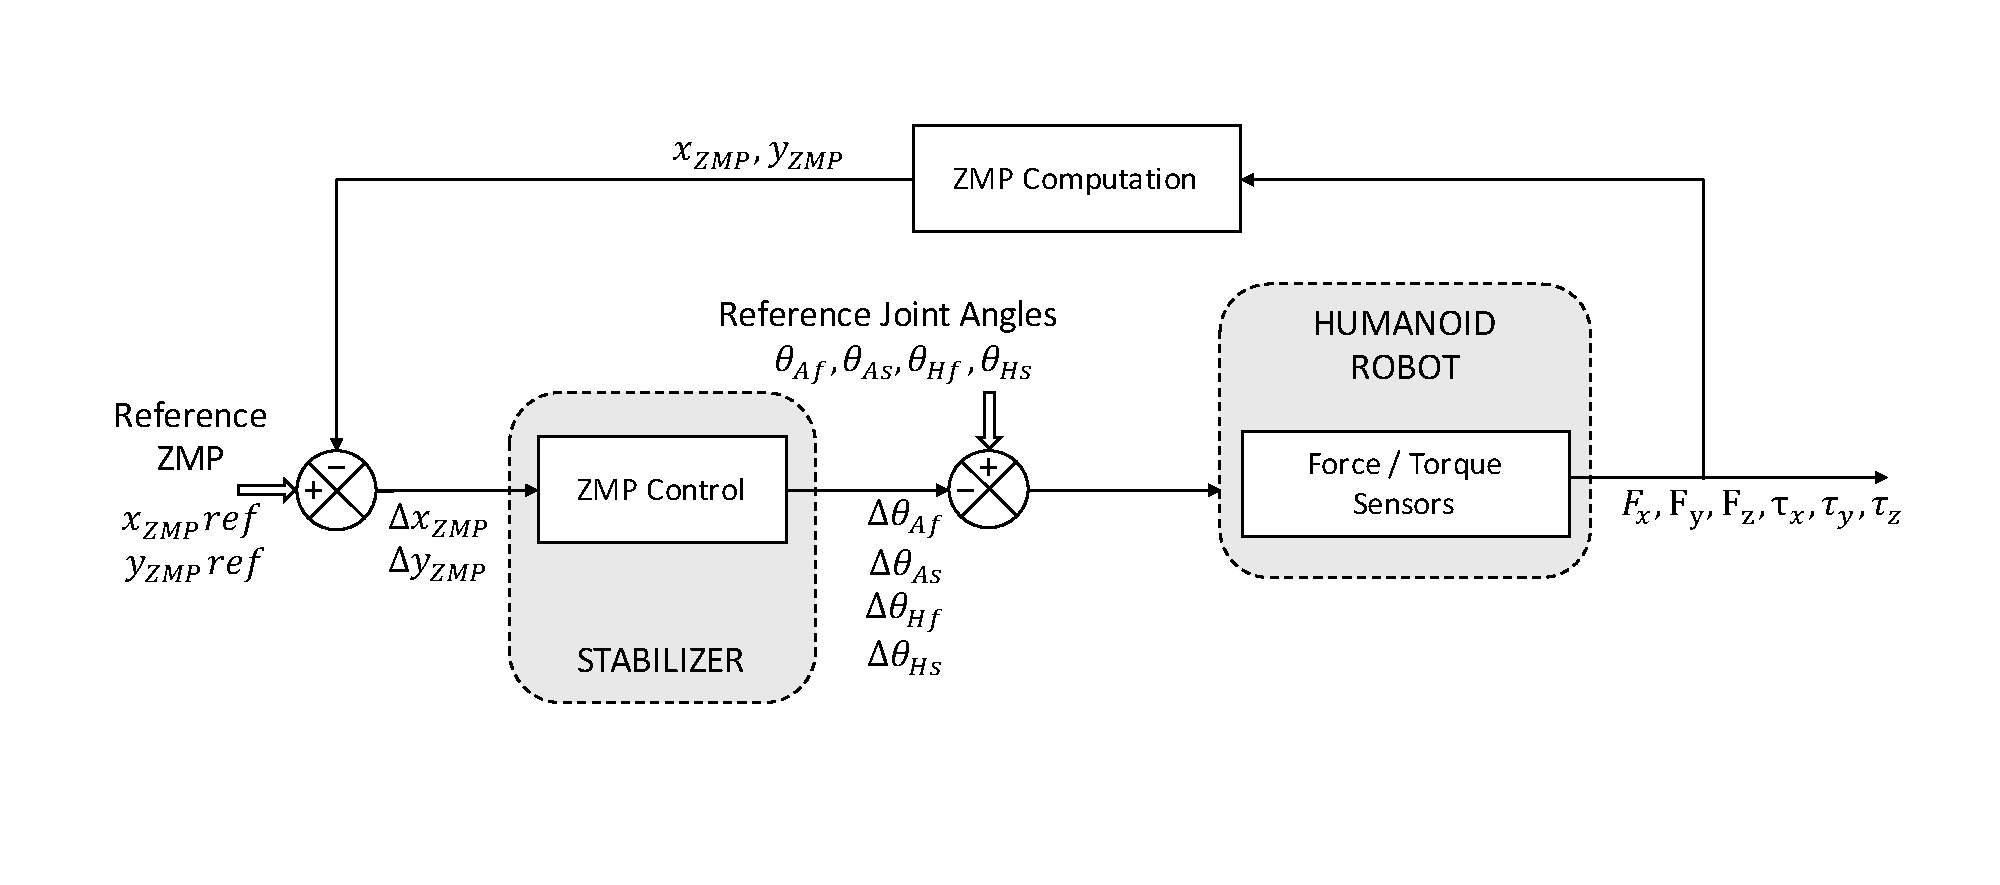
\includegraphics[scale=0.4]{stabilizer.pdf}
\caption{Stabilizer architecture.}
\label{fig:stabilizer}
\end{figure}

The sensorial system of the robot consisting of two six-axis force-torques located at the robot ankles, provides the controller the real distribution of the forces and torques $F_x$, $F_y$, $F_z$, $\tau_x$, $\tau_y$, $\tau_z$ at the contact point of the foot with the ground. After the actual ZMP position $x_{ZMP}$, $y_{ZMP}$ is computed, the ZMP $\Delta x_{ZMP}$, $\Delta y_{ZMP}$ errors can be estimated. These errors are the input data for the Stabilizer and it controls the error in ZMP positioning of the humanoid robot by the motion of the ankle and hip joints.

